\begin{figure}[H]
\centering
%
\begin{subfigure}{0.95\textwidth}
  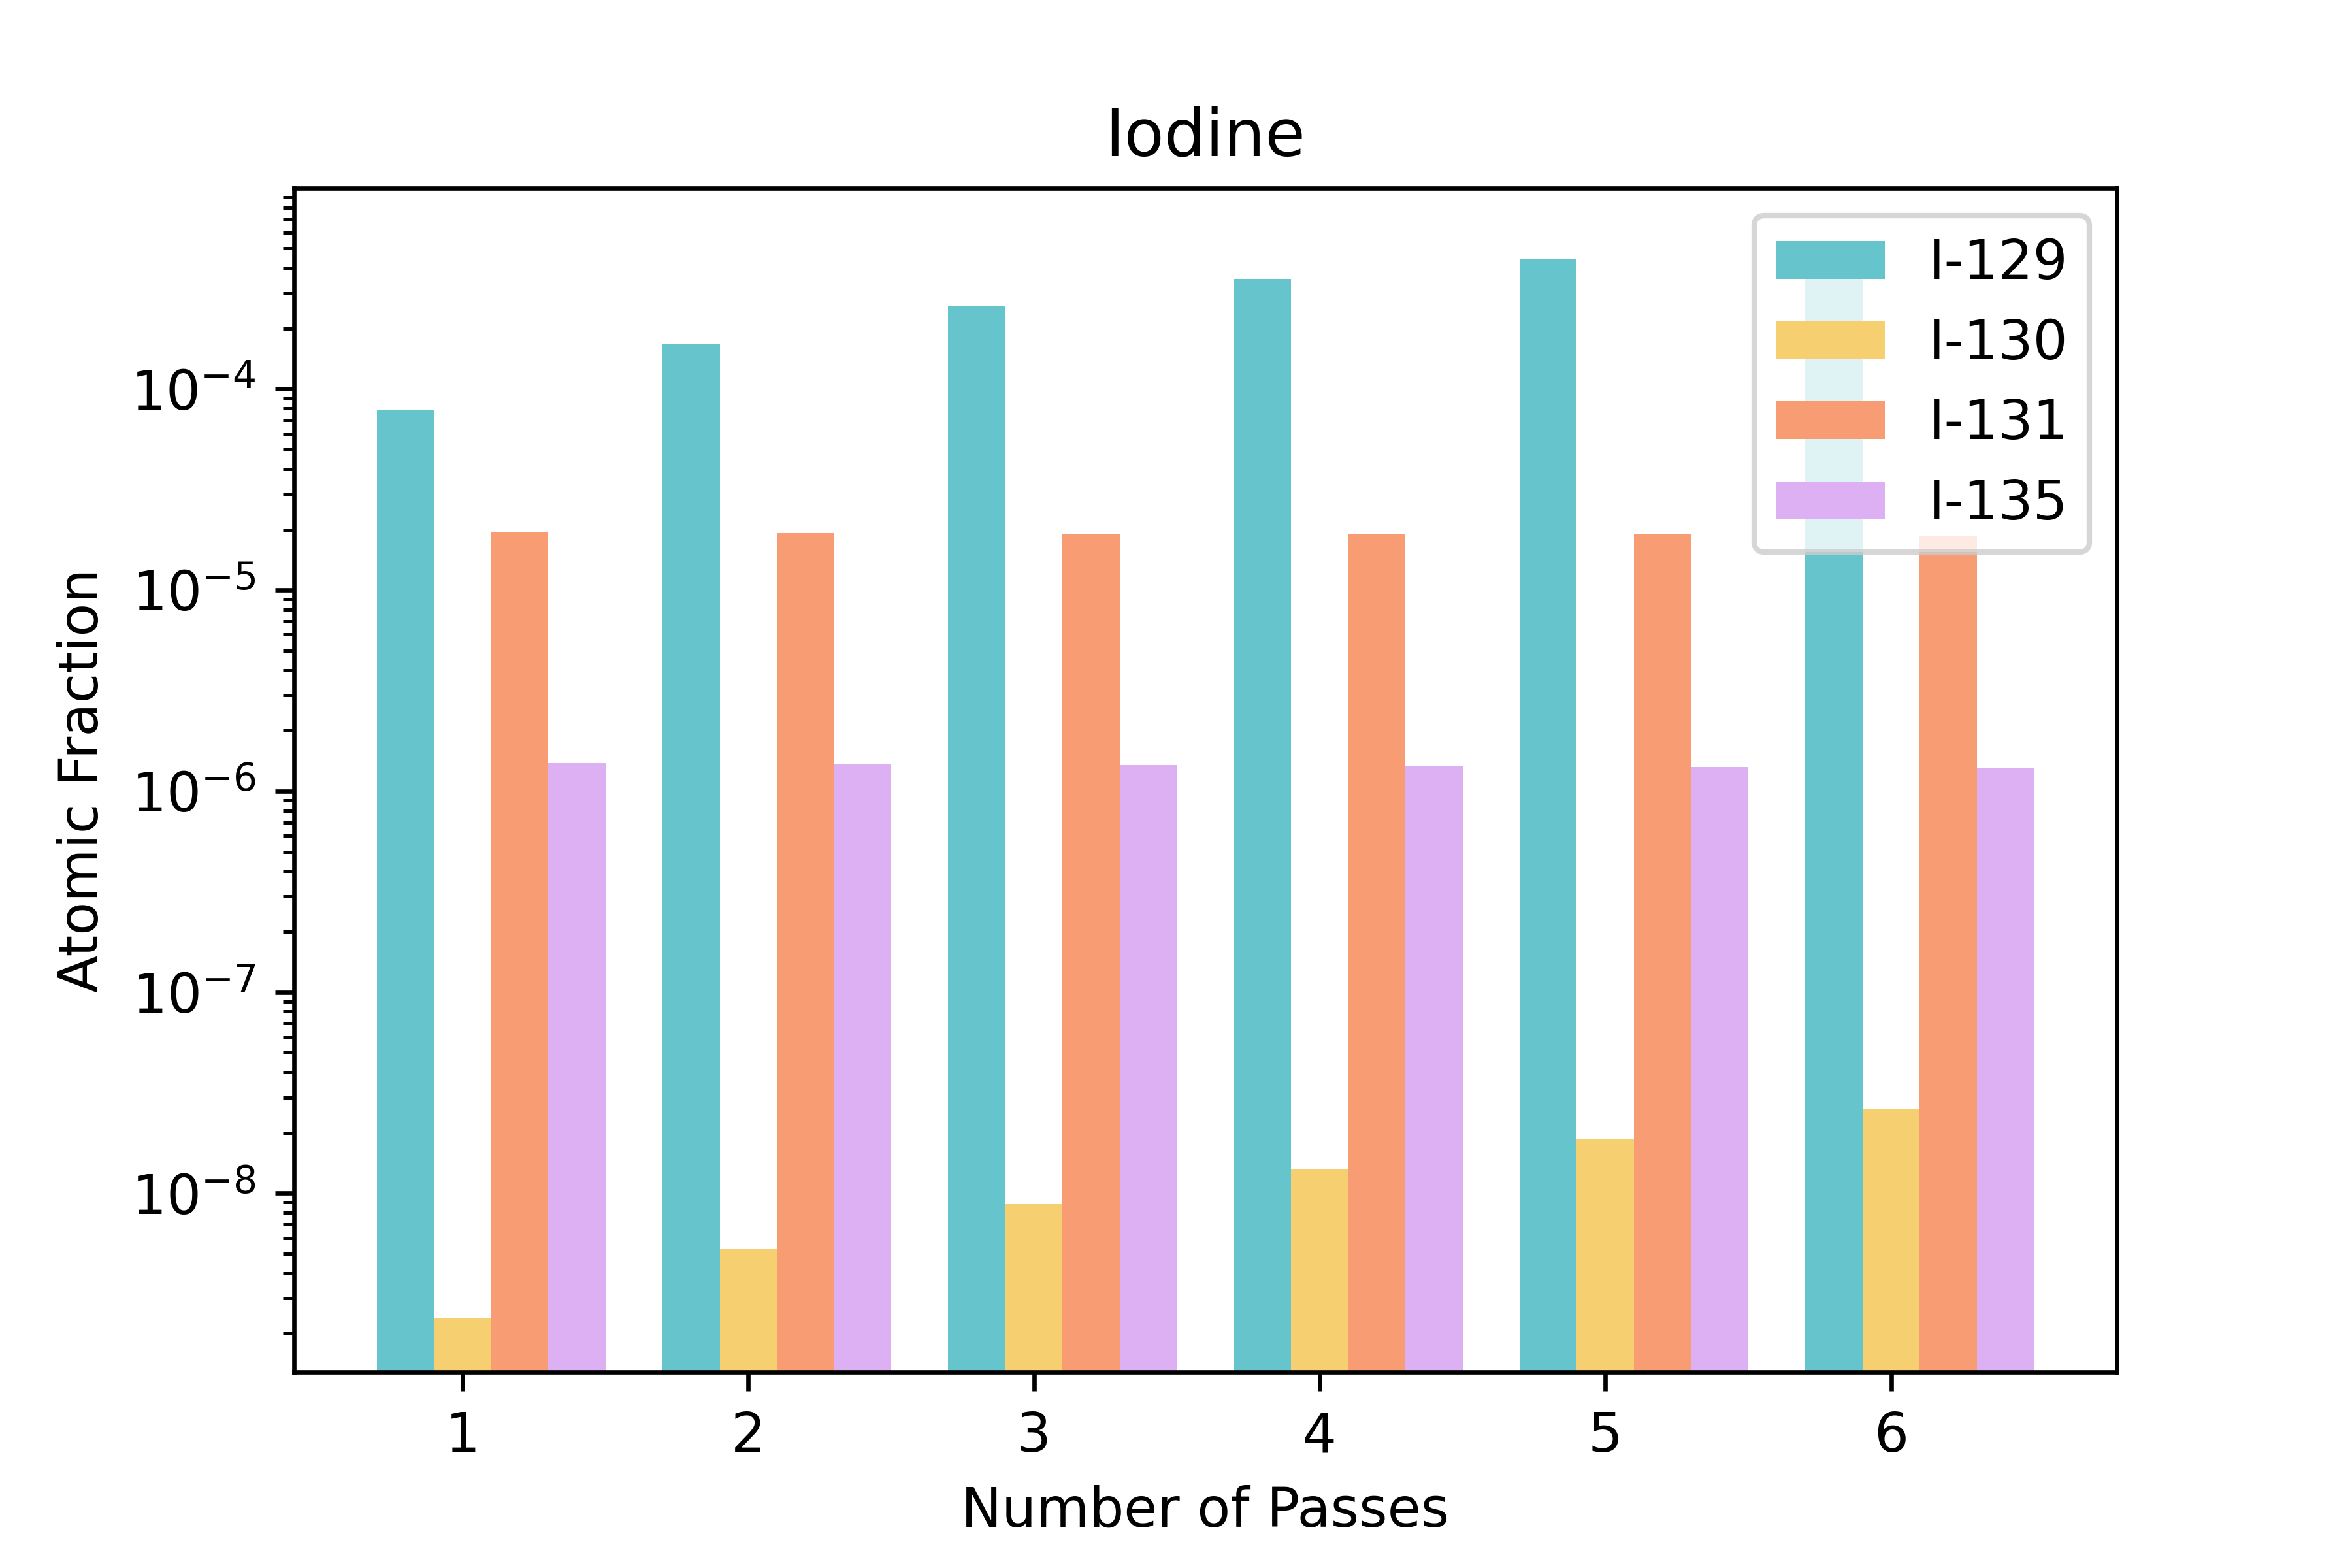
\includegraphics[width=\linewidth]{figures/compositions/iodine}
  \caption{Iodine isotope buildup with each pass}
  \label{fig:i}
\end{subfigure}%

\begin{subfigure}{0.95\textwidth}
  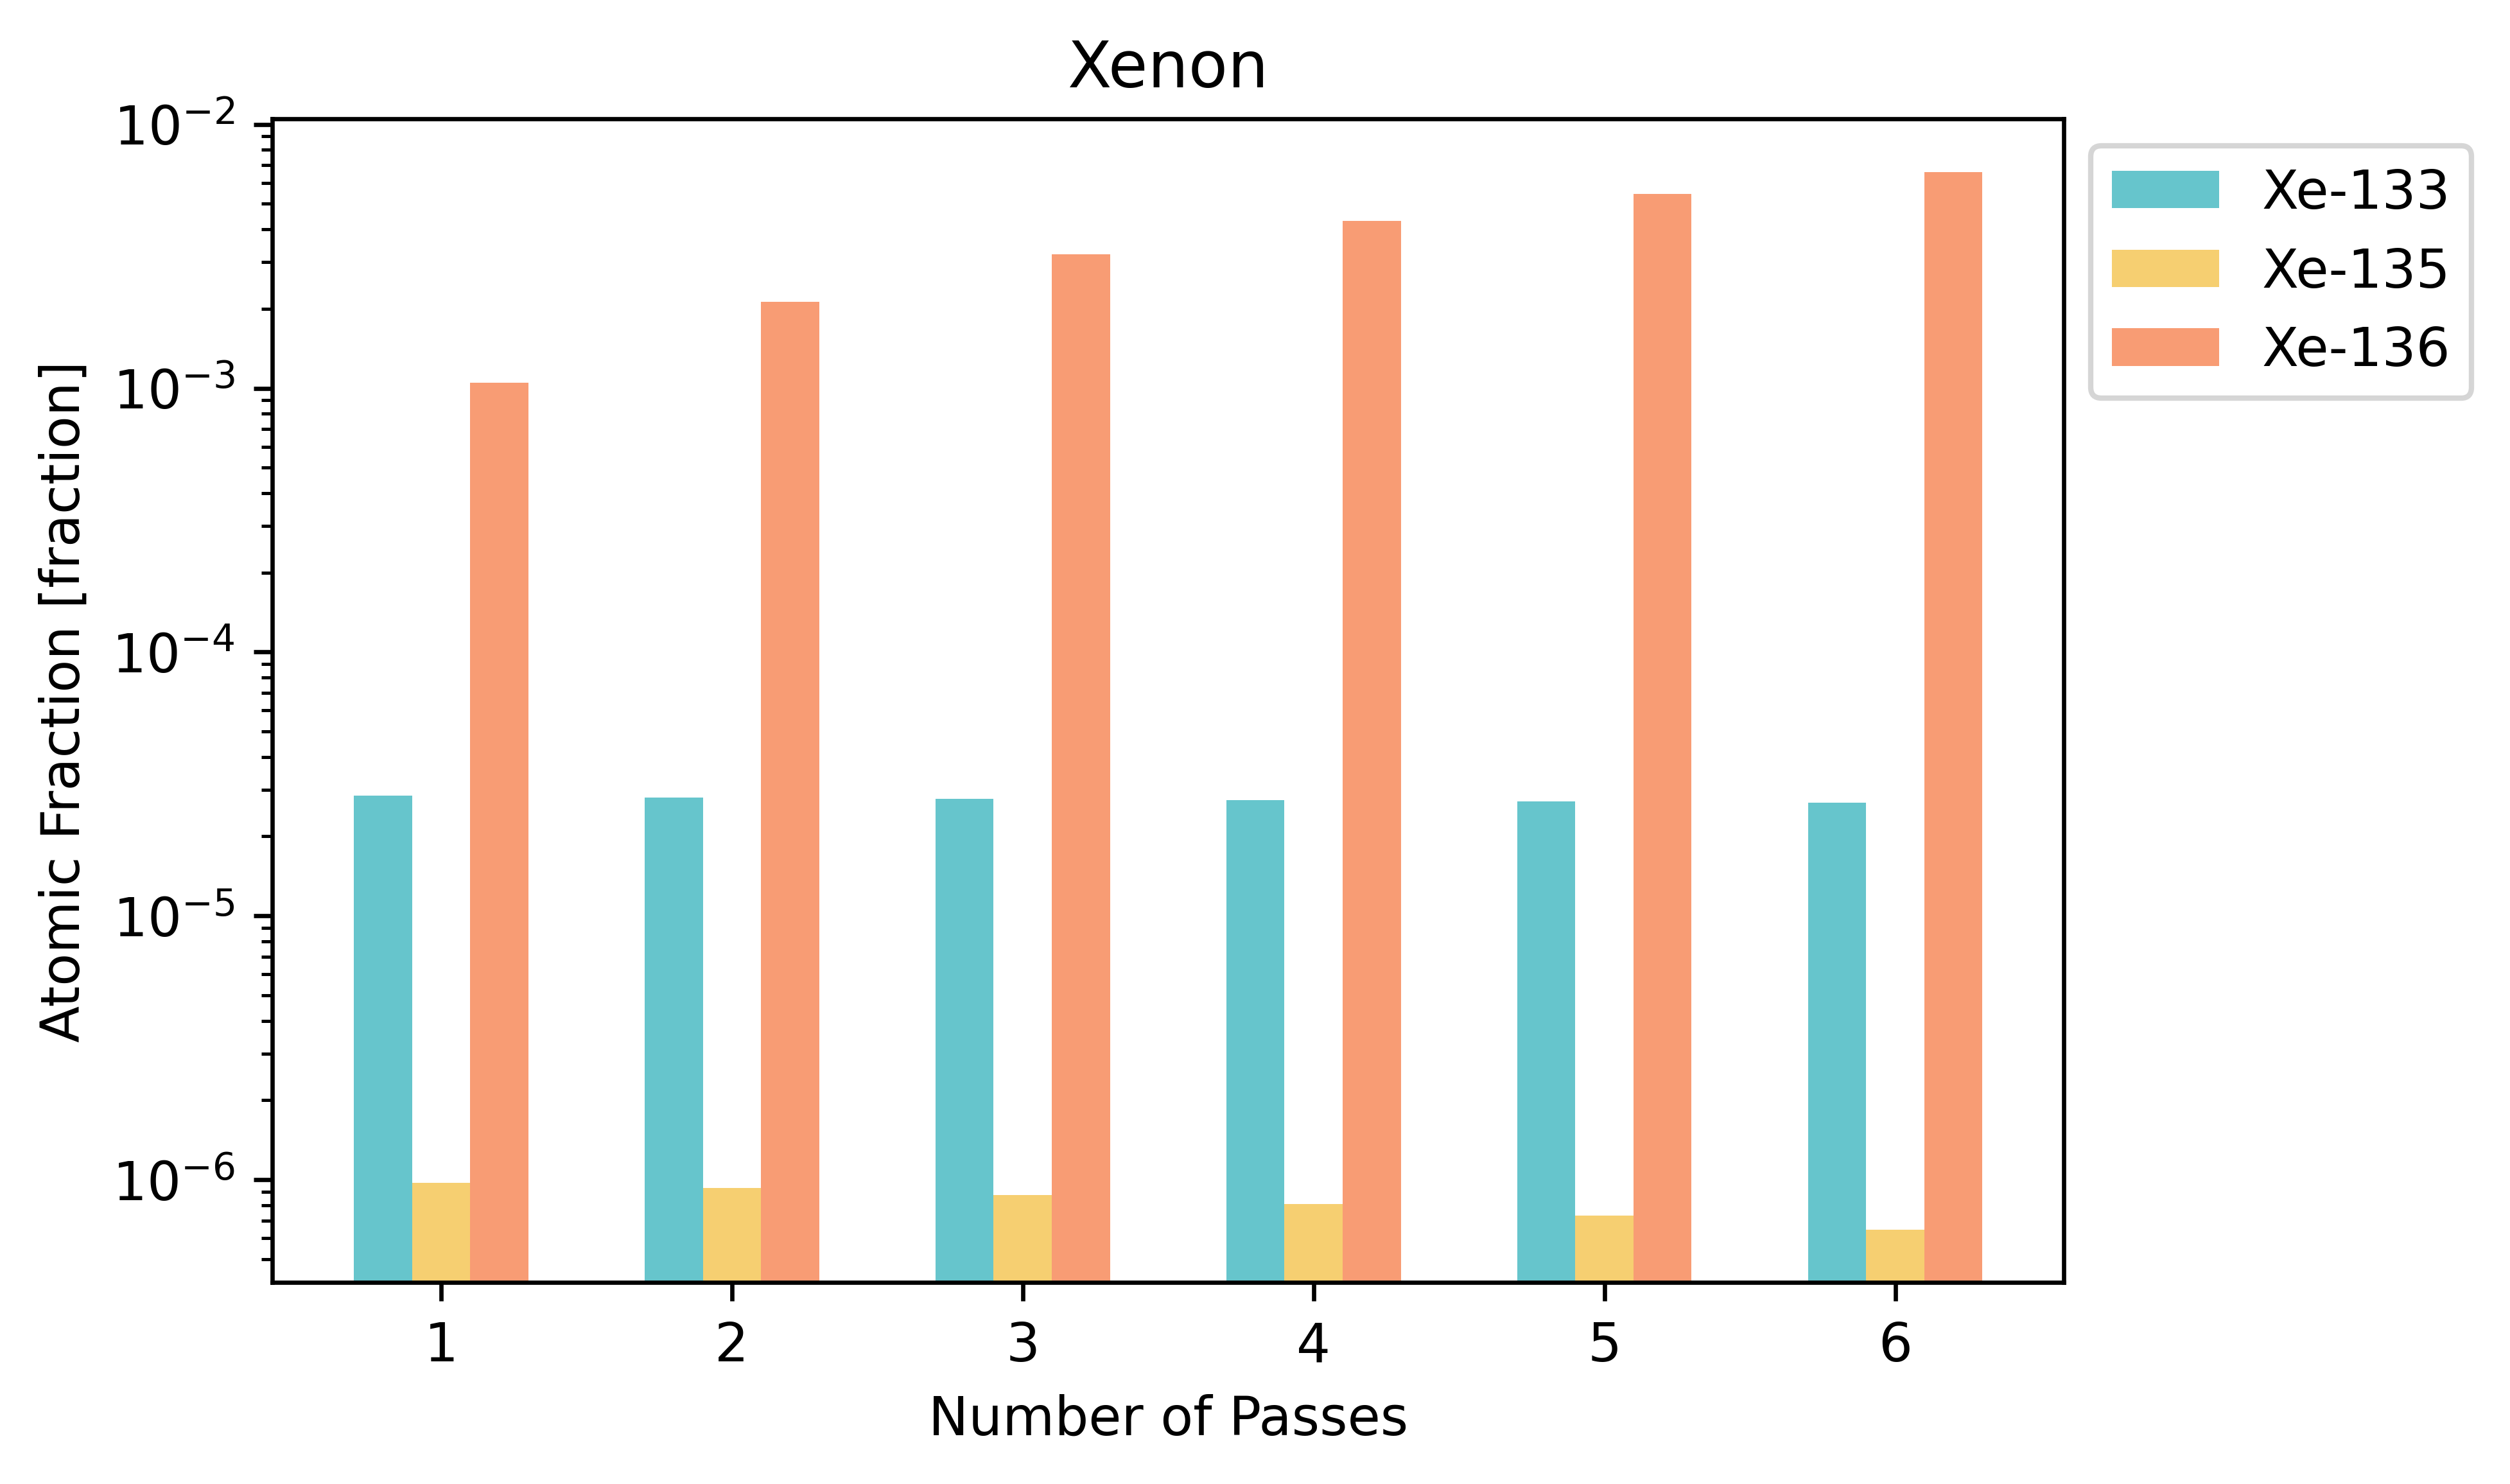
\includegraphics[width=\linewidth]{figures/compositions/xenon}
  \caption{Xenon isotope buildup with each pass}
  \label{fig:xe}
\end{subfigure}%

\caption{Evolution of Safety Relevant Isotopic Concentrations in Pebbles of Sangamon20 over Six Six-Month Passes}
\end{figure}

\begin{figure}[H]\ContinuedFloat
\centering

\begin{subfigure}{0.95\textwidth}
  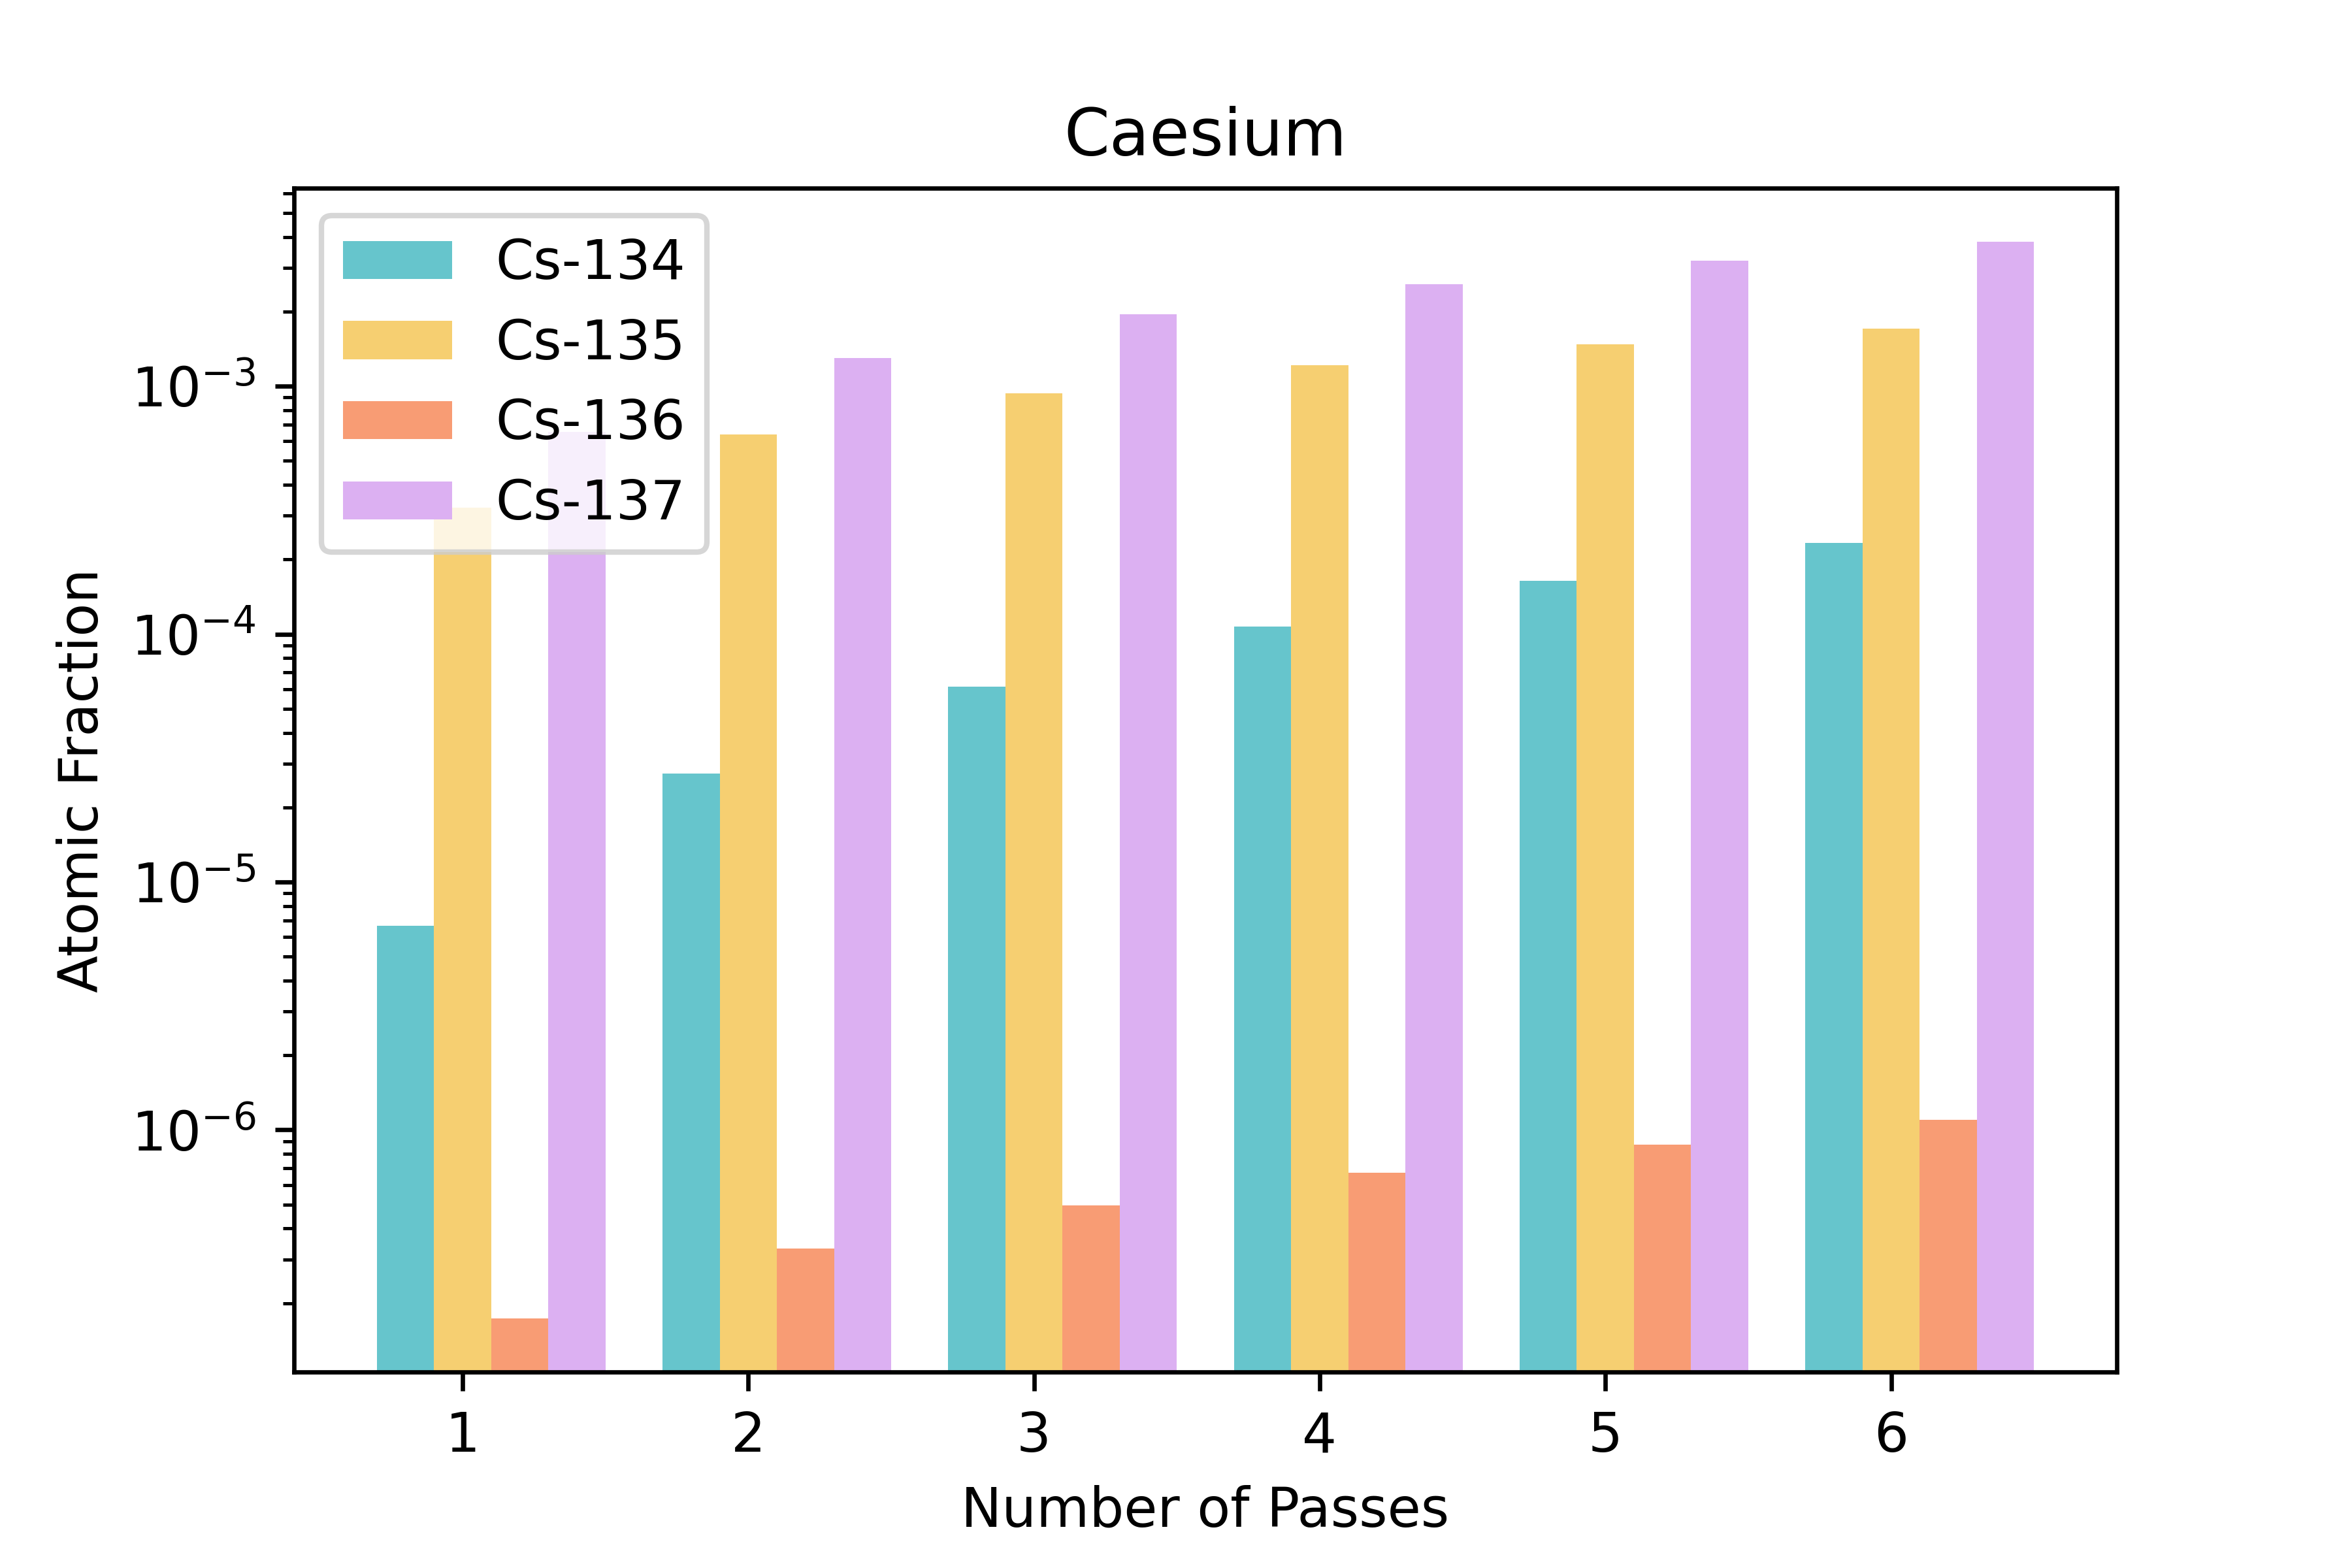
\includegraphics[width=\linewidth]{figures/compositions/caesium}
  \caption{Cesium isotope buildup with each pass}
  \label{fig:cs}
\end{subfigure}%


\begin{subfigure}{0.95\textwidth}
  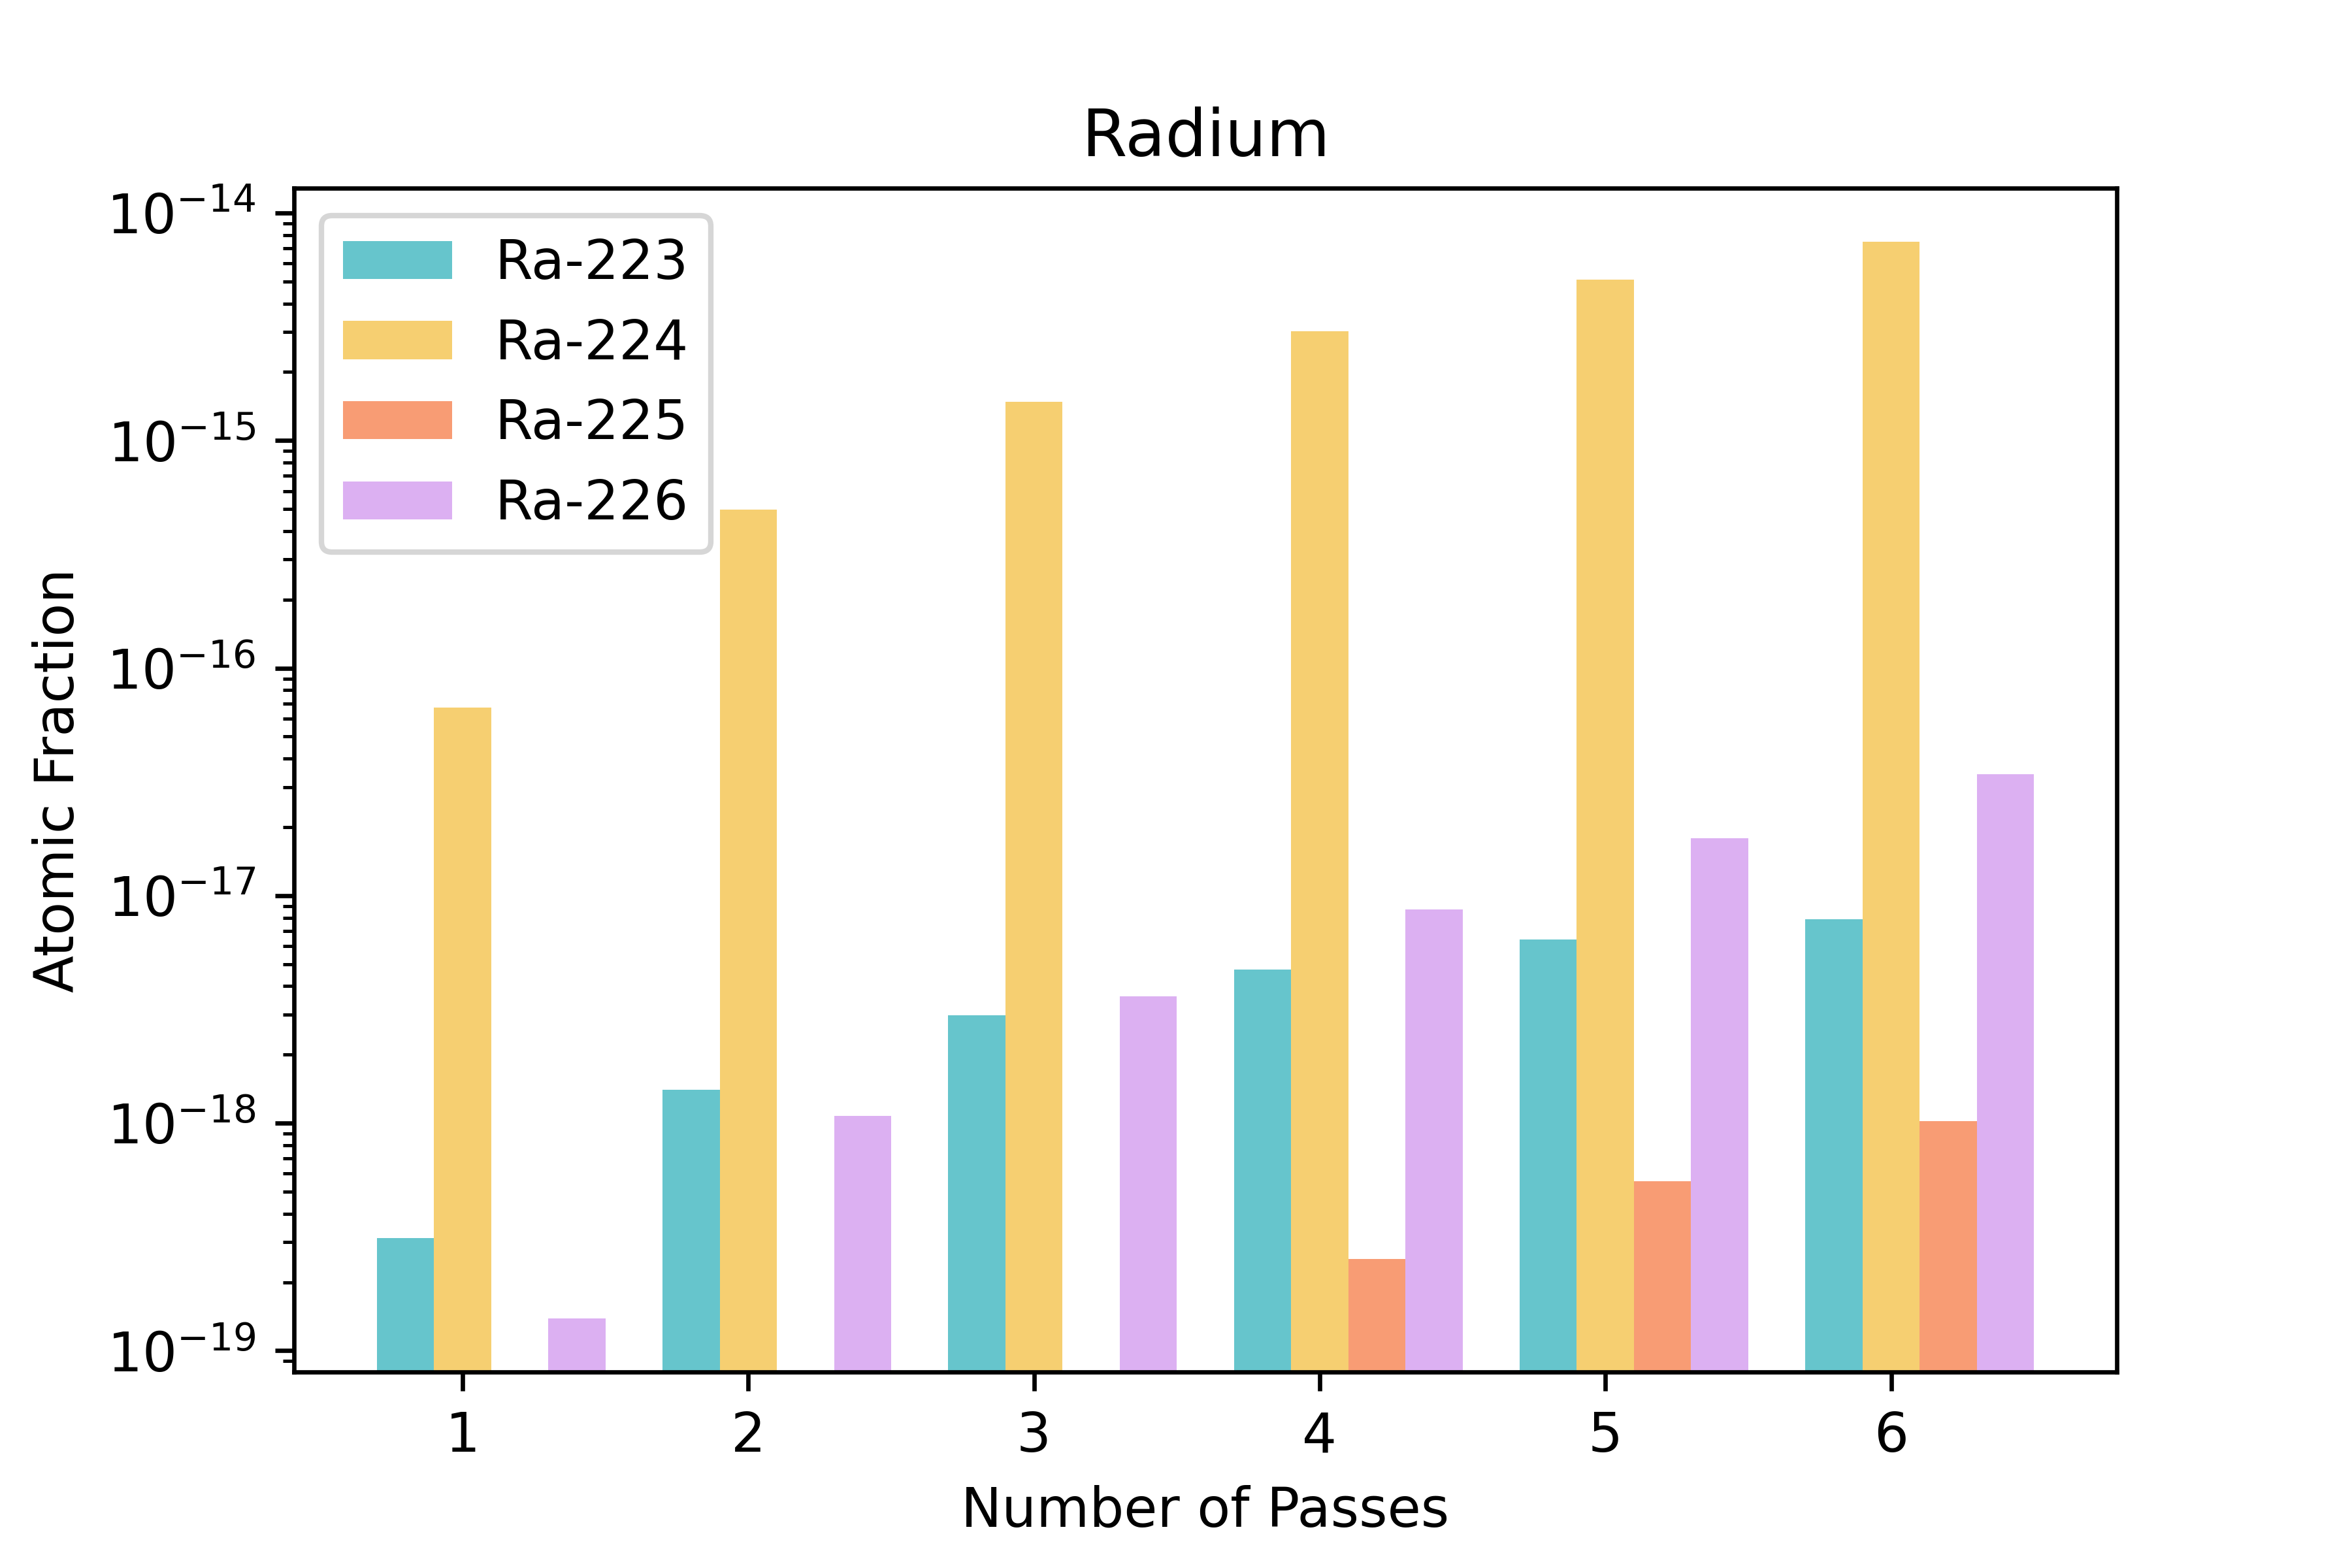
\includegraphics[width=\linewidth]{figures/compositions/radium}
  \caption{Radium isotope buildup with each pass}
  \label{fig:ra}
\end{subfigure}%

\caption{Evolution of Safety Relevant Isotopic Concentrations in Pebbles of Sangamon20 over Six Six-Month Passes (cont.)}
\end{figure}

\begin{figure}[H]\ContinuedFloat
\centering


\begin{subfigure}{0.95\textwidth}
  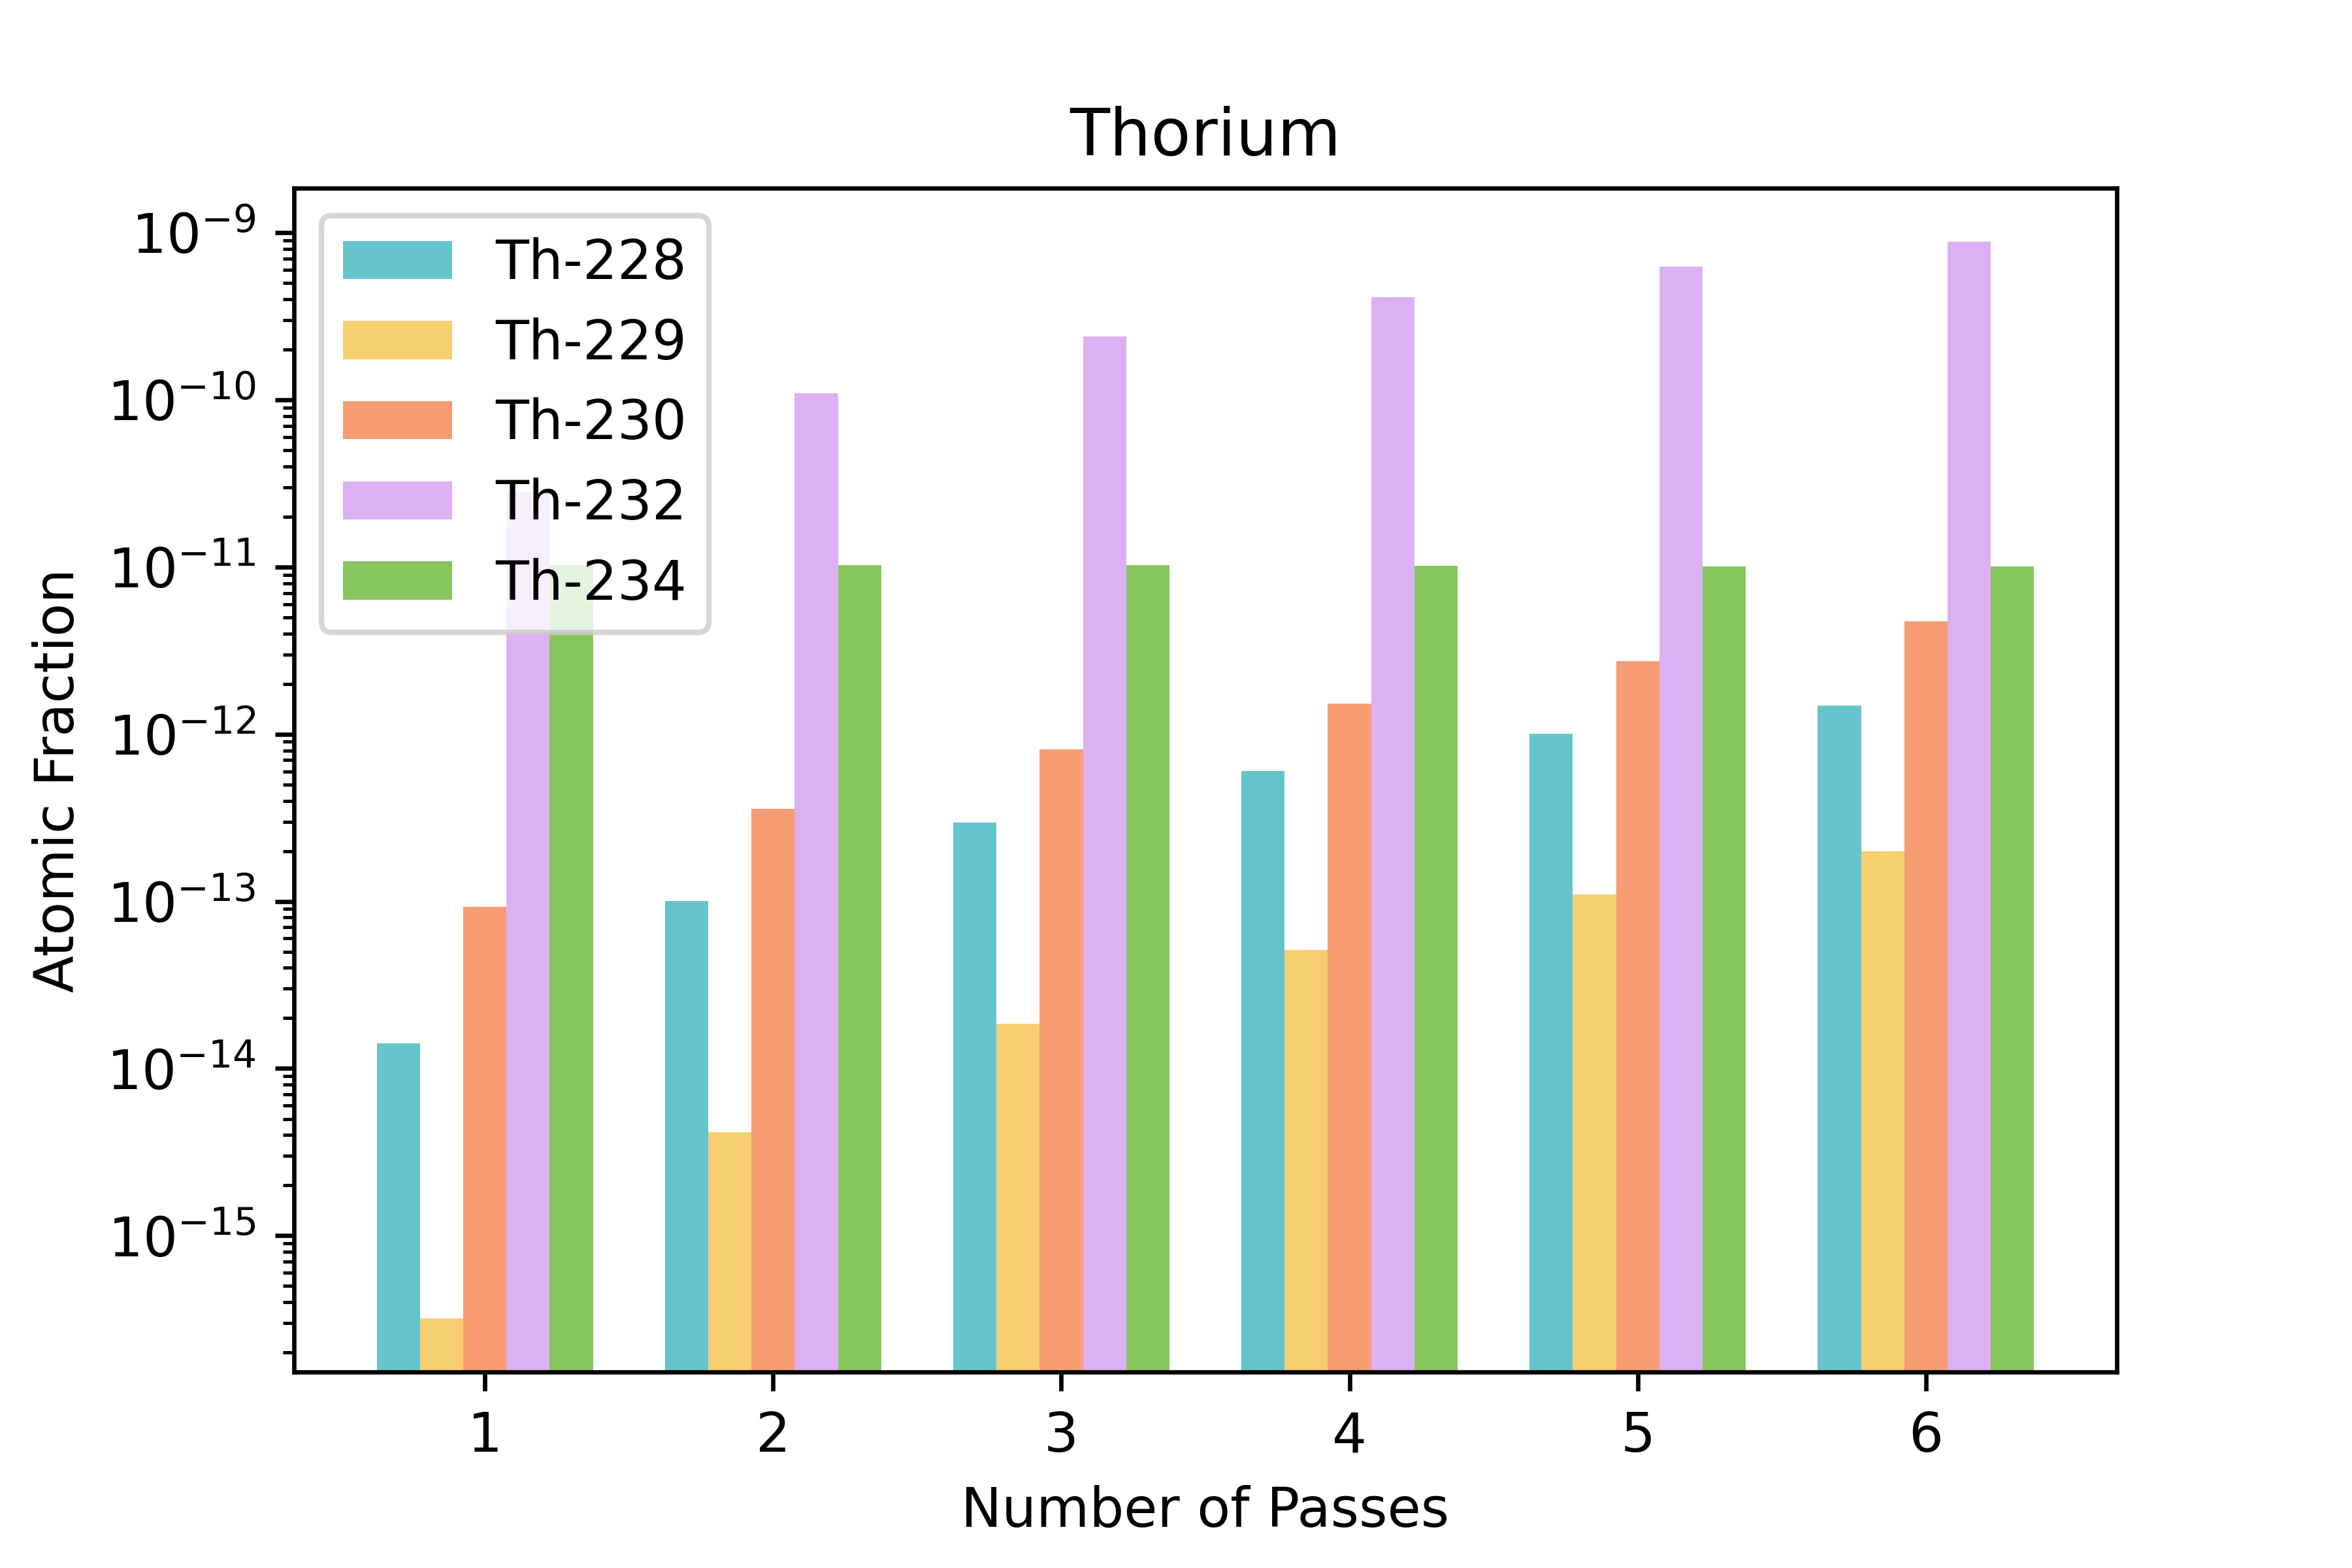
\includegraphics[width=\linewidth]{figures/compositions/thorium}
  \caption{Thorium isotope buildup with each pass}
  \label{fig:th}
\end{subfigure}%

\begin{subfigure}{0.95\textwidth}
  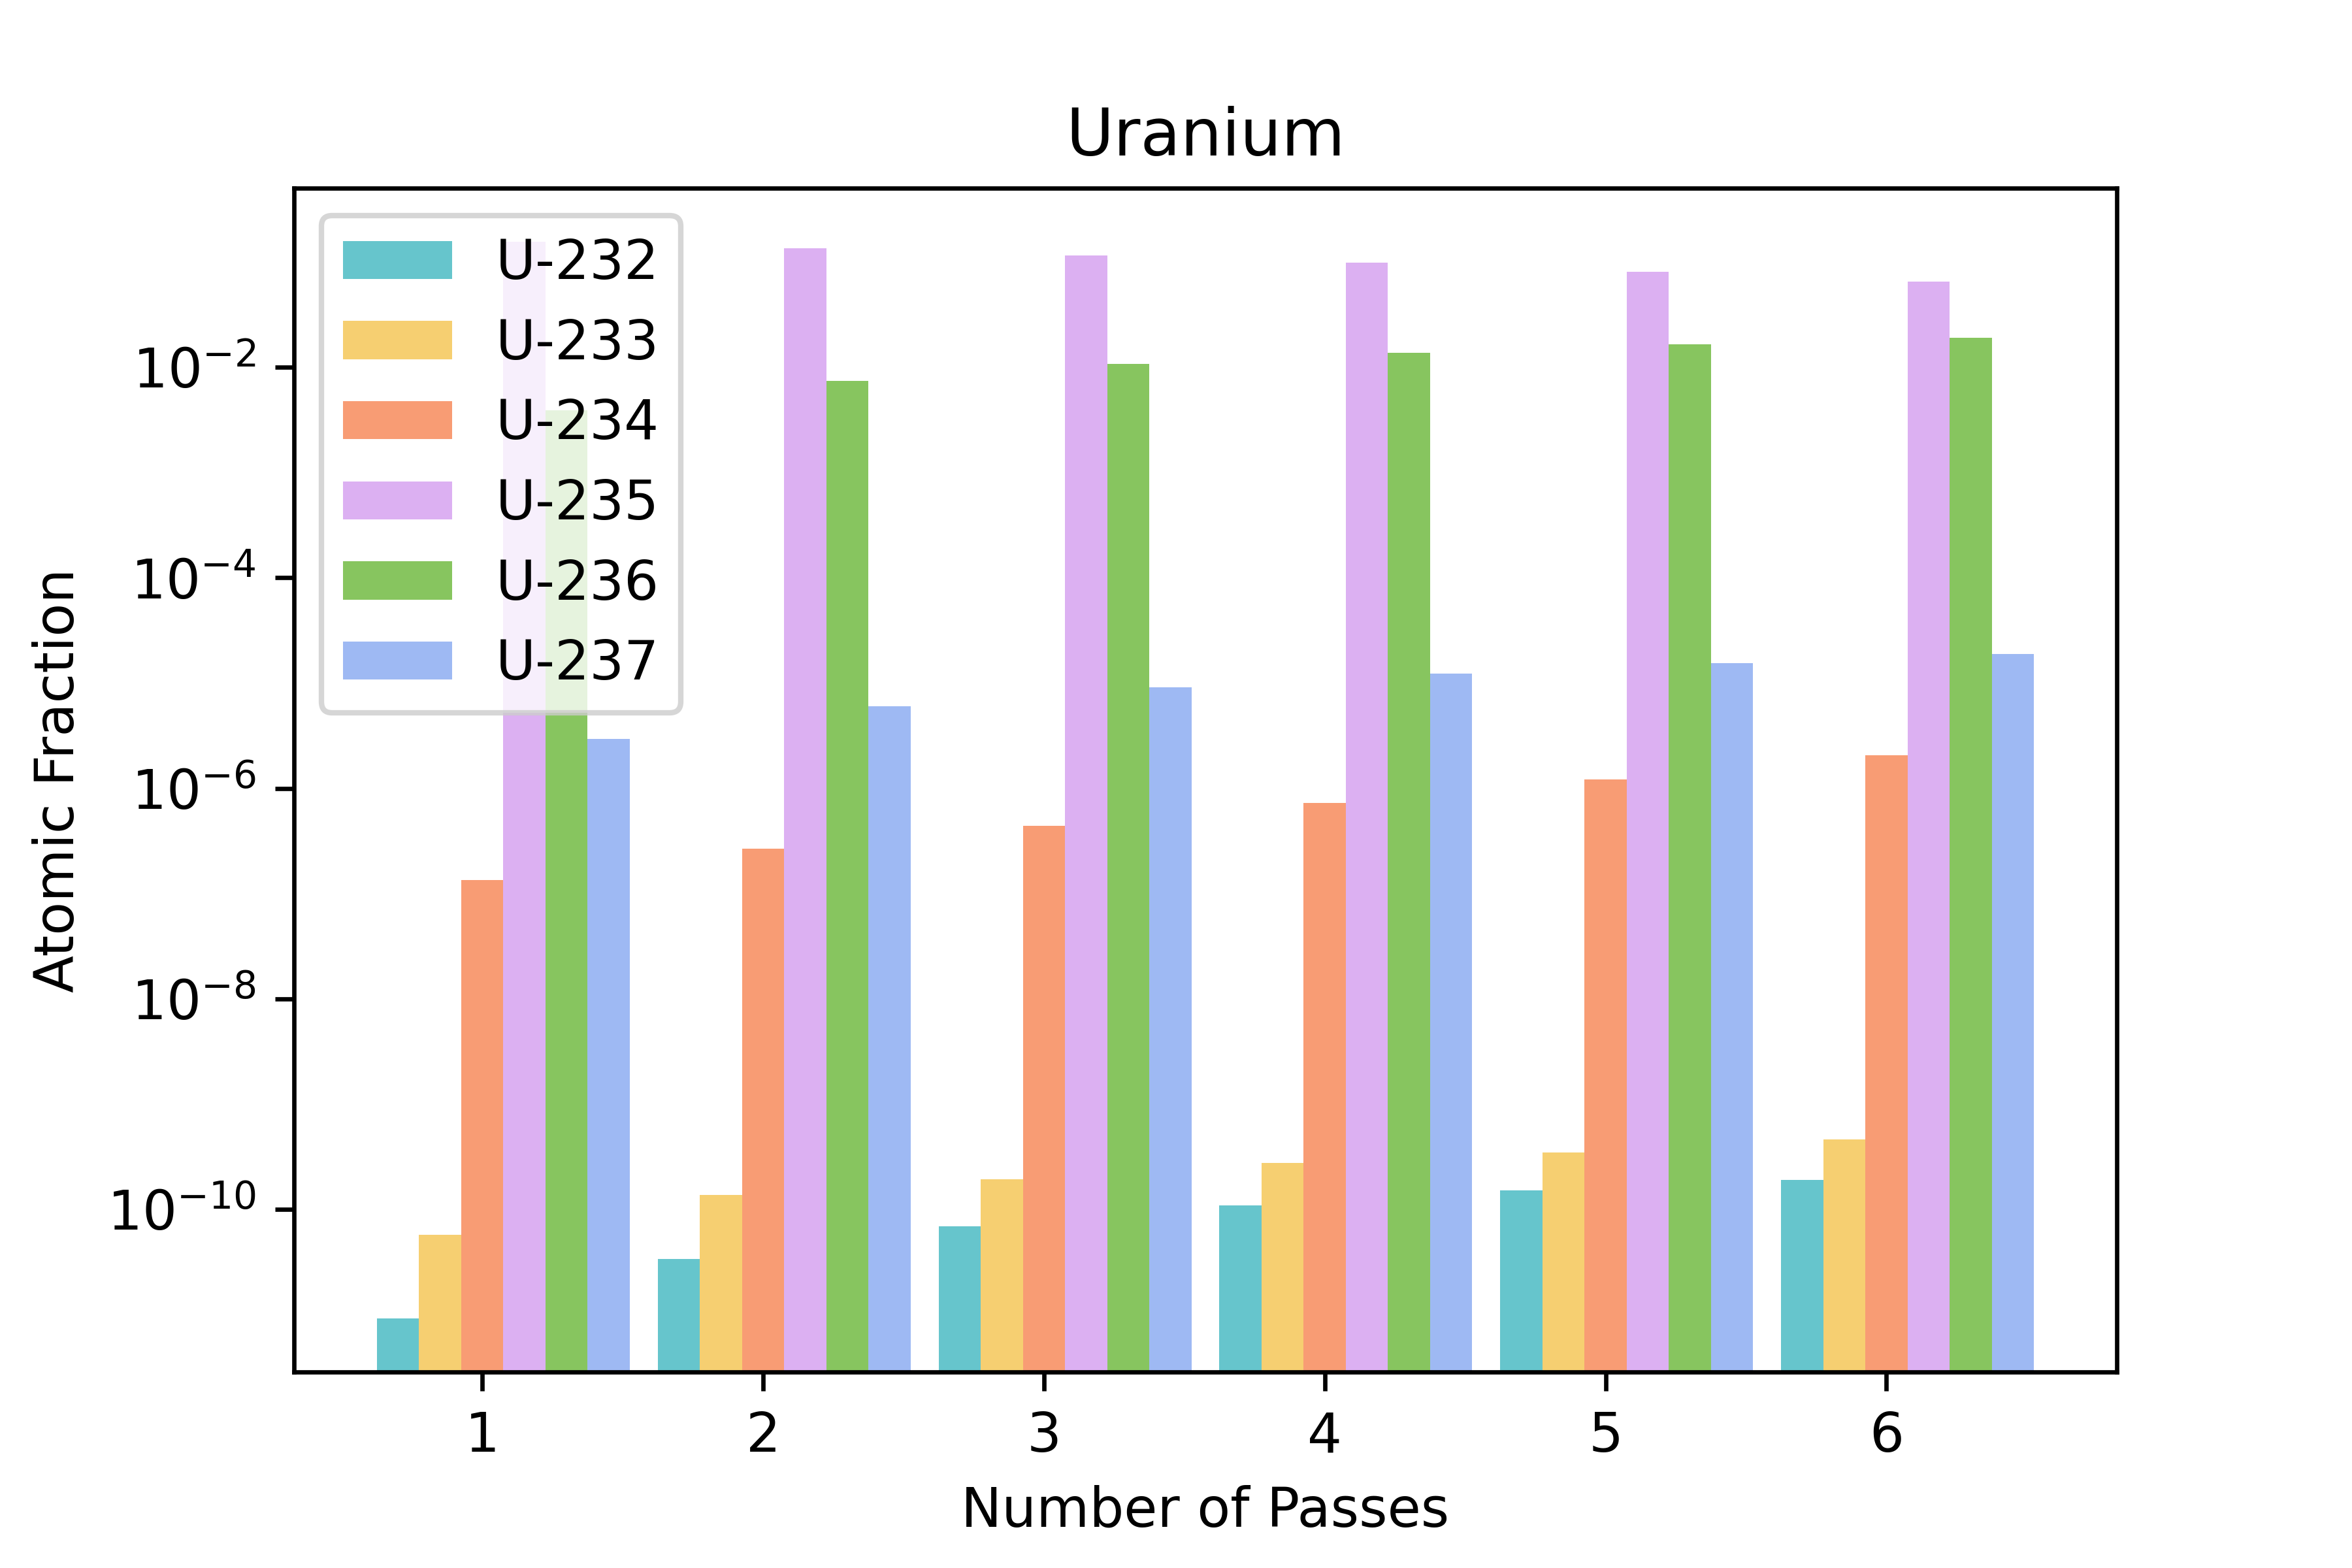
\includegraphics[width=\linewidth]{figures/compositions/uranium}
  \caption{Uranium isotope buildup with each pass}
  \label{fig:u}
\end{subfigure}%

\caption{Evolution of Safety Relevant Isotopic Concentrations in Pebbles of Sangamon20 over Six Six-Month Passes (cont.)}
\end{figure}

\begin{figure}[H]\ContinuedFloat
\centering

\begin{subfigure}{0.95\textwidth}
  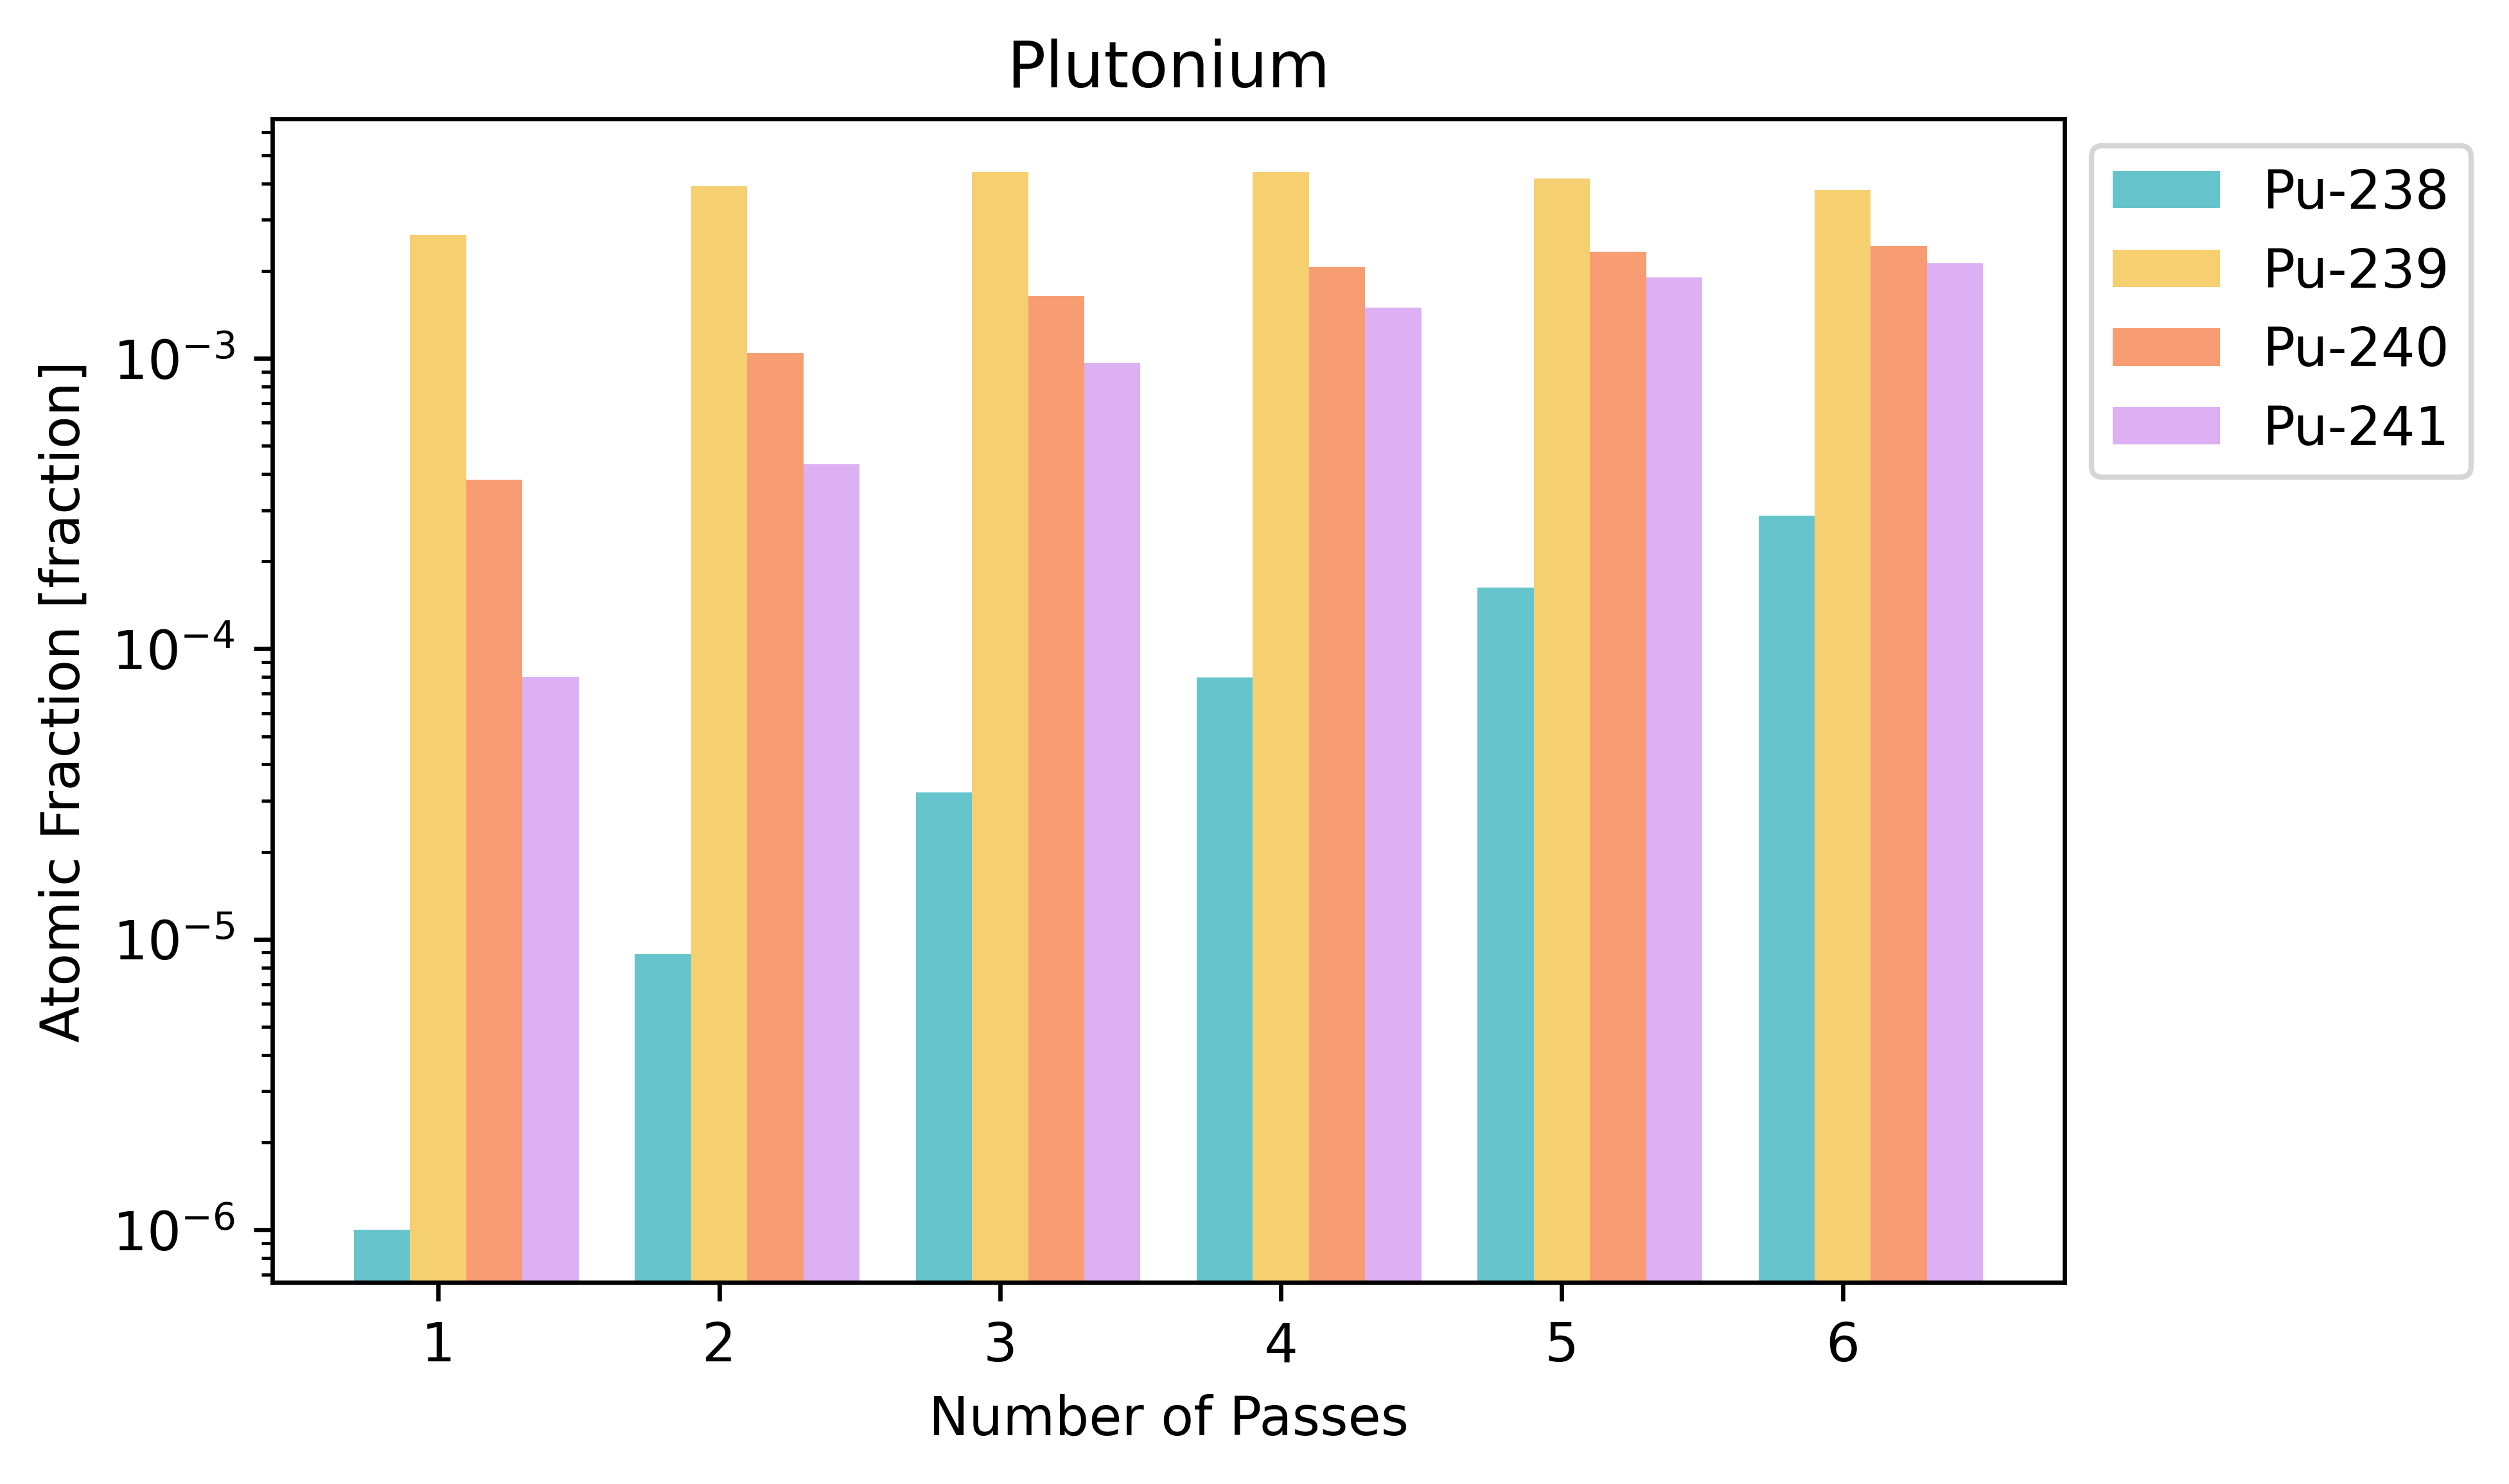
\includegraphics[width=\linewidth]{figures/compositions/plutonium}
  \caption{Plutonium isotope buildup with each pass}
  \label{fig:pu}
\end{subfigure}%

\caption{Evolution of Certain Isotopic Concentrations in Pebbles over Six Six-Month Passes (cont.)}
\label{fig:comps}
\end{figure}